\documentclass[multi=page, border=0.5cm]{standalone}
\usepackage{calculator}
\usepackage[svgnames]{xcolor}
\usepackage{tikz}
\usetikzlibrary{patterns}

% defining the new dimensions and parameters
\newlength{\hatchspread}
\newlength{\hatchthickness}
\newlength{\hatchshift}
\newcommand{\hatchcolor}{}
% declaring the keys in tikz
\tikzset{hatchspread/.code={\setlength{\hatchspread}{#1}},
         hatchthickness/.code={\setlength{\hatchthickness}{#1}},
         hatchshift/.code={\setlength{\hatchshift}{#1}},% must be >= 0
         hatchcolor/.code={\renewcommand{\hatchcolor}{#1}}}
% setting the default values
\tikzset{hatchspread=3pt,
         hatchthickness=0.4pt,
         hatchshift=0pt,% must be >= 0
         hatchcolor=black}
% declaring the pattern
\pgfdeclarepatternformonly[\hatchspread,\hatchthickness,\hatchshift,\hatchcolor]% variables
   {custom north west lines}% name
   {\pgfqpoint{\dimexpr-2\hatchthickness}{\dimexpr-2\hatchthickness}}% lower left corner
   {\pgfqpoint{\dimexpr\hatchspread+2\hatchthickness}{\dimexpr\hatchspread+2\hatchthickness}}% upper right corner
   {\pgfqpoint{\dimexpr\hatchspread}{\dimexpr\hatchspread}}% tile size
   {% shape description
    \pgfsetlinewidth{\hatchthickness}
    \pgfpathmoveto{\pgfqpoint{0pt}{\dimexpr\hatchspread+\hatchshift}}
    \pgfpathlineto{\pgfqpoint{\dimexpr\hatchspread+0.15pt+\hatchshift}{-0.15pt}}
    \ifdim \hatchshift > 0pt
      \pgfpathmoveto{\pgfqpoint{0pt}{\hatchshift}}
      \pgfpathlineto{\pgfqpoint{\dimexpr0.15pt+\hatchshift}{-0.15pt}}
    \fi
    \pgfsetstrokecolor{\hatchcolor}
%    \pgfsetdash{{1pt}{1pt}}{0pt}% dashing cannot work correctly in all situation this way
    \pgfusepath{stroke}
   }
   
\tikzset{    
    poly/.style={ line width=2mm, red },
    shadow1/.style={ black, opacity=0.15, fill },
    shadow2/.style={ black, opacity=0.25, fill }
}


\begin{document}
\begin{page}
    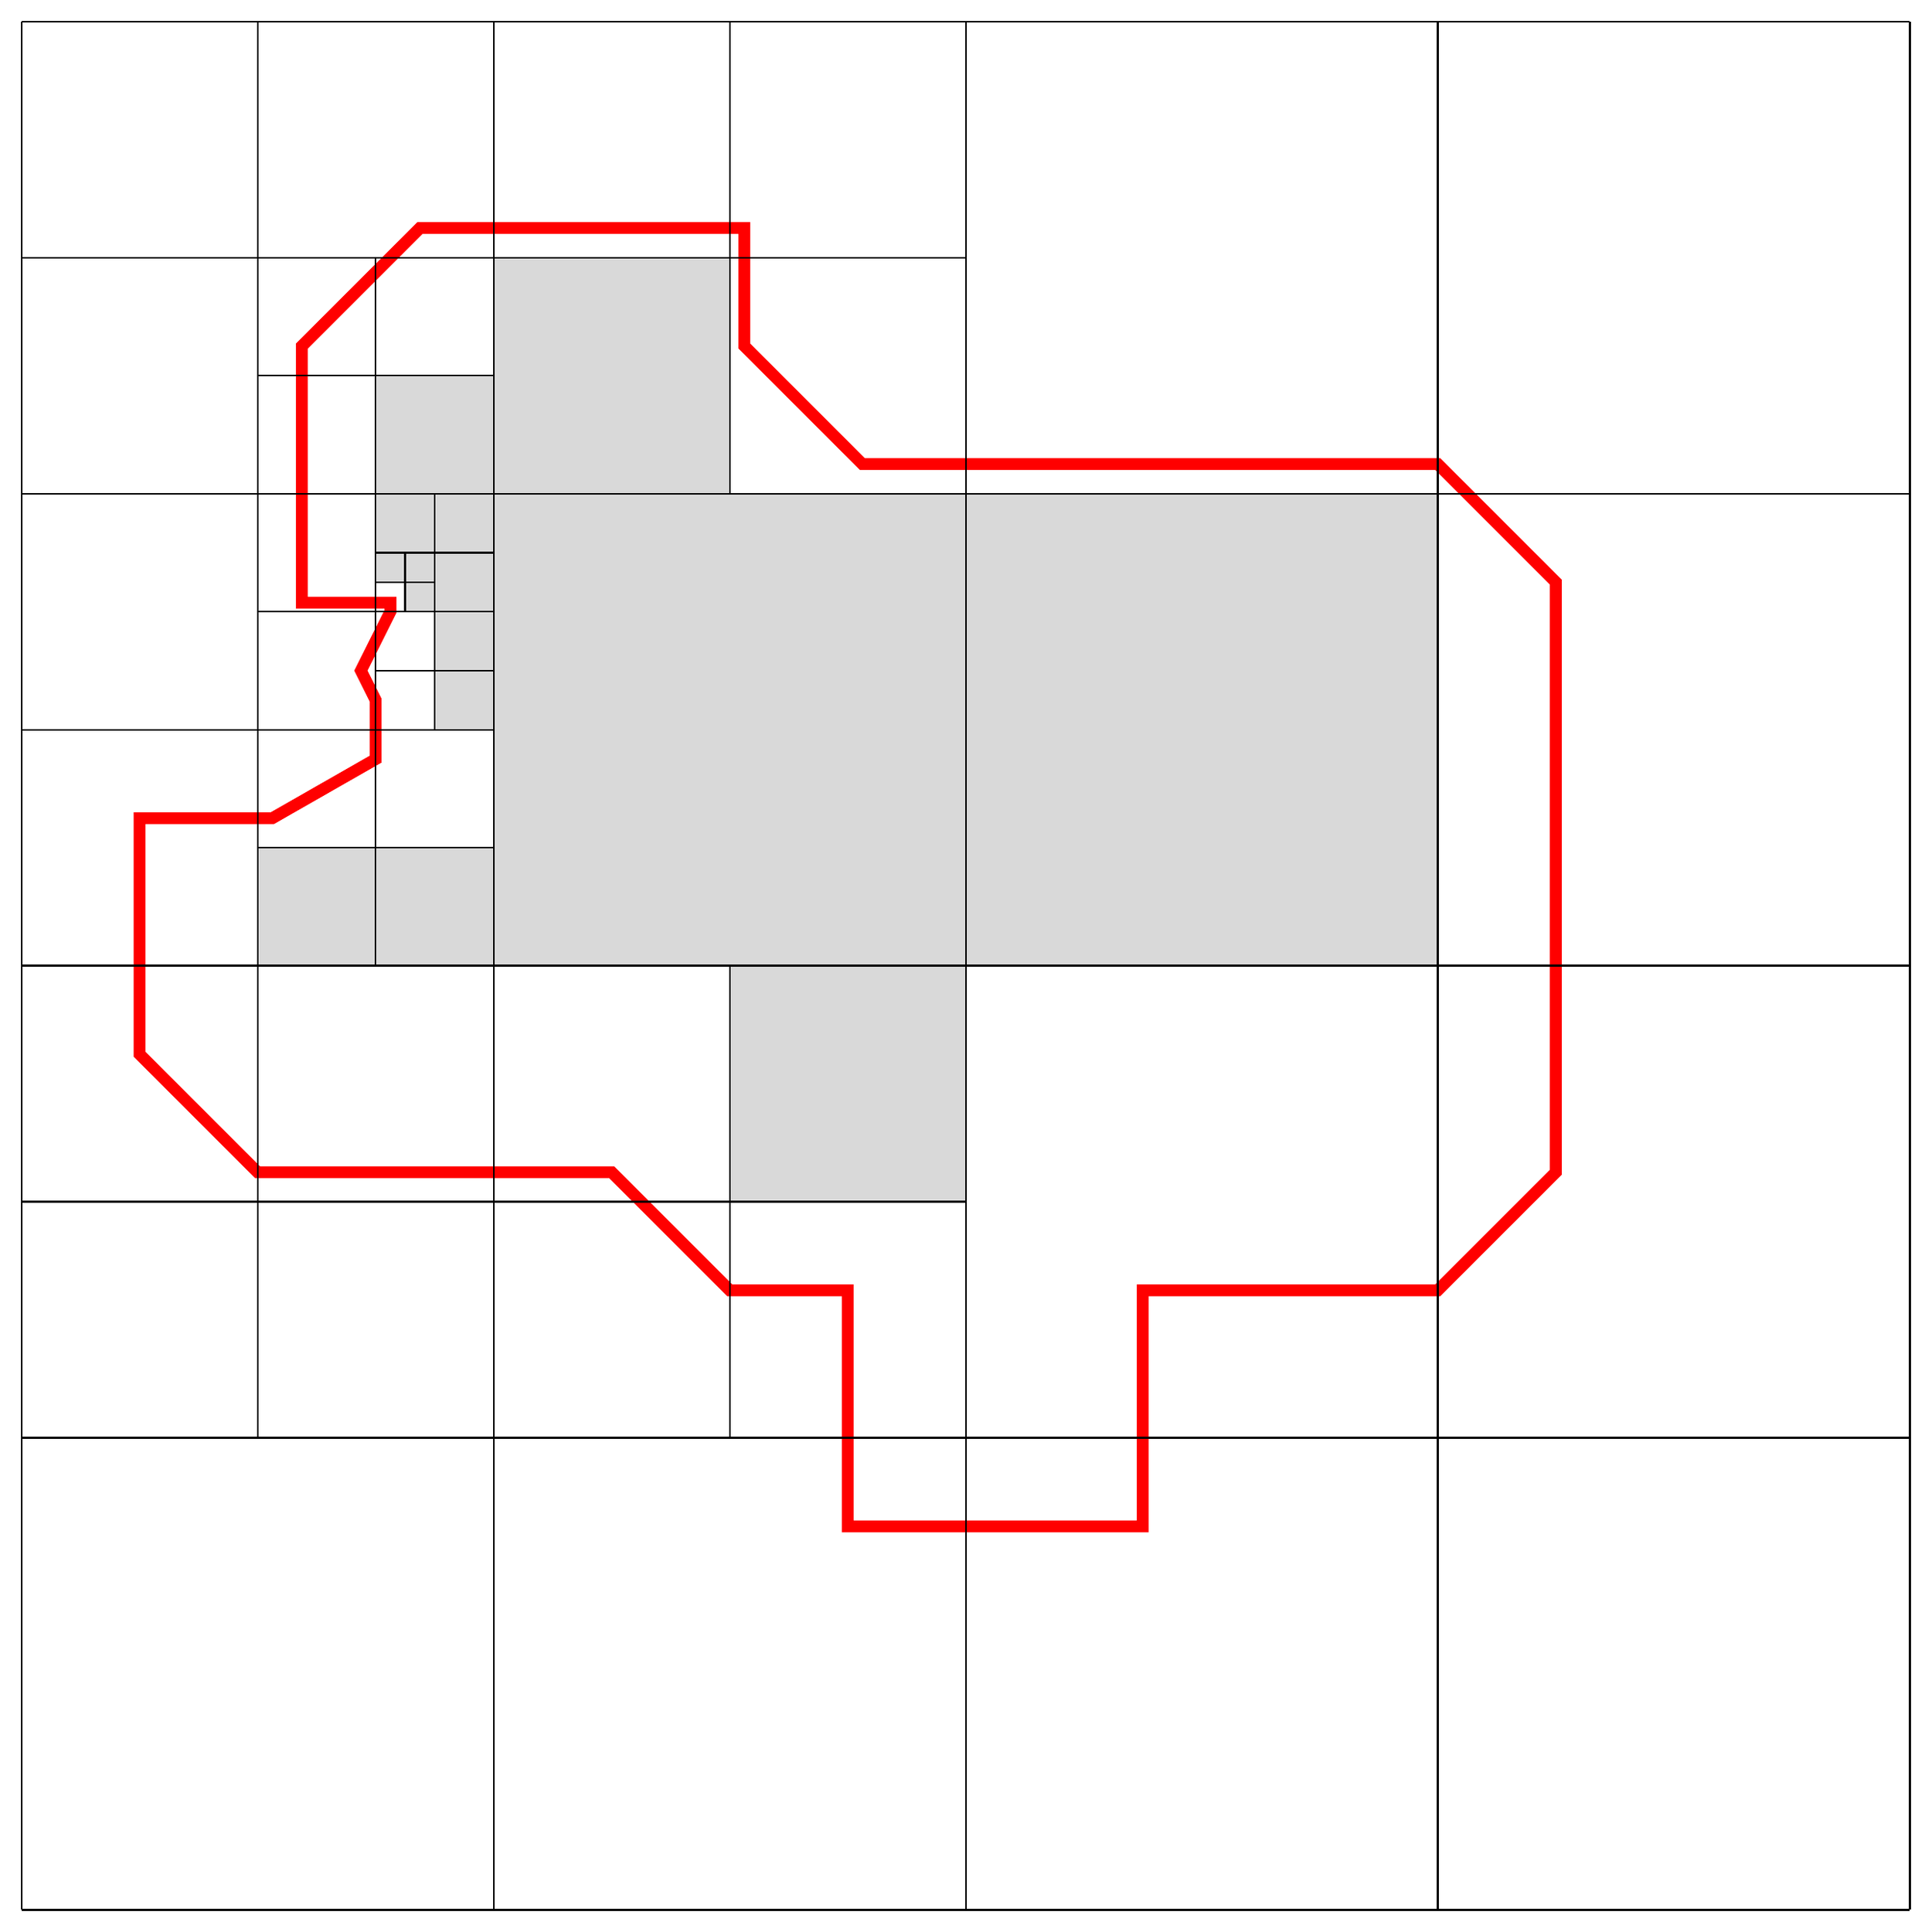
\begin{tikzpicture}
        %\draw[step=1, very thin, light-gray, dashed] (0,0) grid (32,32);
        
        \node (start) at (6.25,22.25) {};
        \draw[poly] (start) -- ++(0,-0.25) -- ++(-0.25,-0.5) -- ++(-0.25,-0.5)  -- ++(0.25,-0.5)
            -- ++(0,-1) -- ++(-1.75,-1) -- ++(-2.25,0) -- ++(0,-4) -- ++(2,-2)
            -- ++(6,0) -- ++(2,-2) -- ++(2,0) -- ++(0,-4) -- ++(5,0) -- ++(0,4) -- ++(5,0) 
            -- ++(2,2) -- ++(0,10) -- ++(-2,2) -- ++(-9.75,0) -- ++(-2,2) 
            -- ++(0,2) -- ++(-5.5,0) -- ++(-2,-2) -- ++(0,-4.35) -- ++(1.6,0);
        \draw[step=8,  thick, black] (0,0)  grid (32,32);
        \draw[step=4,  thick, black] (0,24) grid (8,32);
        \draw[step=4,  thick, black] (0,16) grid (8,24);
        \draw[step=4,  thick, black] (0,8)  grid (8,16);
        \draw[step=4,  thick, black] (8,8)  grid (16,16);
        \draw[step=4,  thick, black] (8,24) grid (16,32);
        \draw[step=2,  thick, black] (4,16) grid (8,20);
        \draw[step=2,  thick, black] (4,20) grid (8,24);
        \draw[step=2,  thick, black] (4,24) grid (8,28);
        \draw[step=1,  thick, black] (6,20) grid (8,24);
        \draw[step=0.5,thick, black] (6,22) grid (7,23);

        \draw[shadow1] (8,16) rectangle (16,24);
        \draw[shadow1] (16,16) rectangle (24,24);
        \draw[shadow1] (6,16) rectangle (8,18);
        \draw[shadow1] (4,16) rectangle (6,18);
        \draw[shadow1] (12,12) rectangle (16,16);
        \draw[shadow1] (8,24) rectangle (12,28);
        \draw[shadow1] (6,24) rectangle (8,26);        
        \draw[shadow1] (6,23) rectangle (7,24);
        \draw[shadow1] (7,23) rectangle (8,24);
        \draw[shadow1] (7,22) rectangle (8,23);
        \draw[shadow1] (7,21) rectangle (8,22);
        \draw[shadow1] (7,20) rectangle (8,21);
        \draw[shadow1] (6,22.5) rectangle (6.5,23);
        \draw[shadow1] (6.5,22.5) rectangle (7,23);
        \draw[shadow1] (6.5,22) rectangle (7,22.5);
        
    \end{tikzpicture}
\end{page}

\begin{page}
    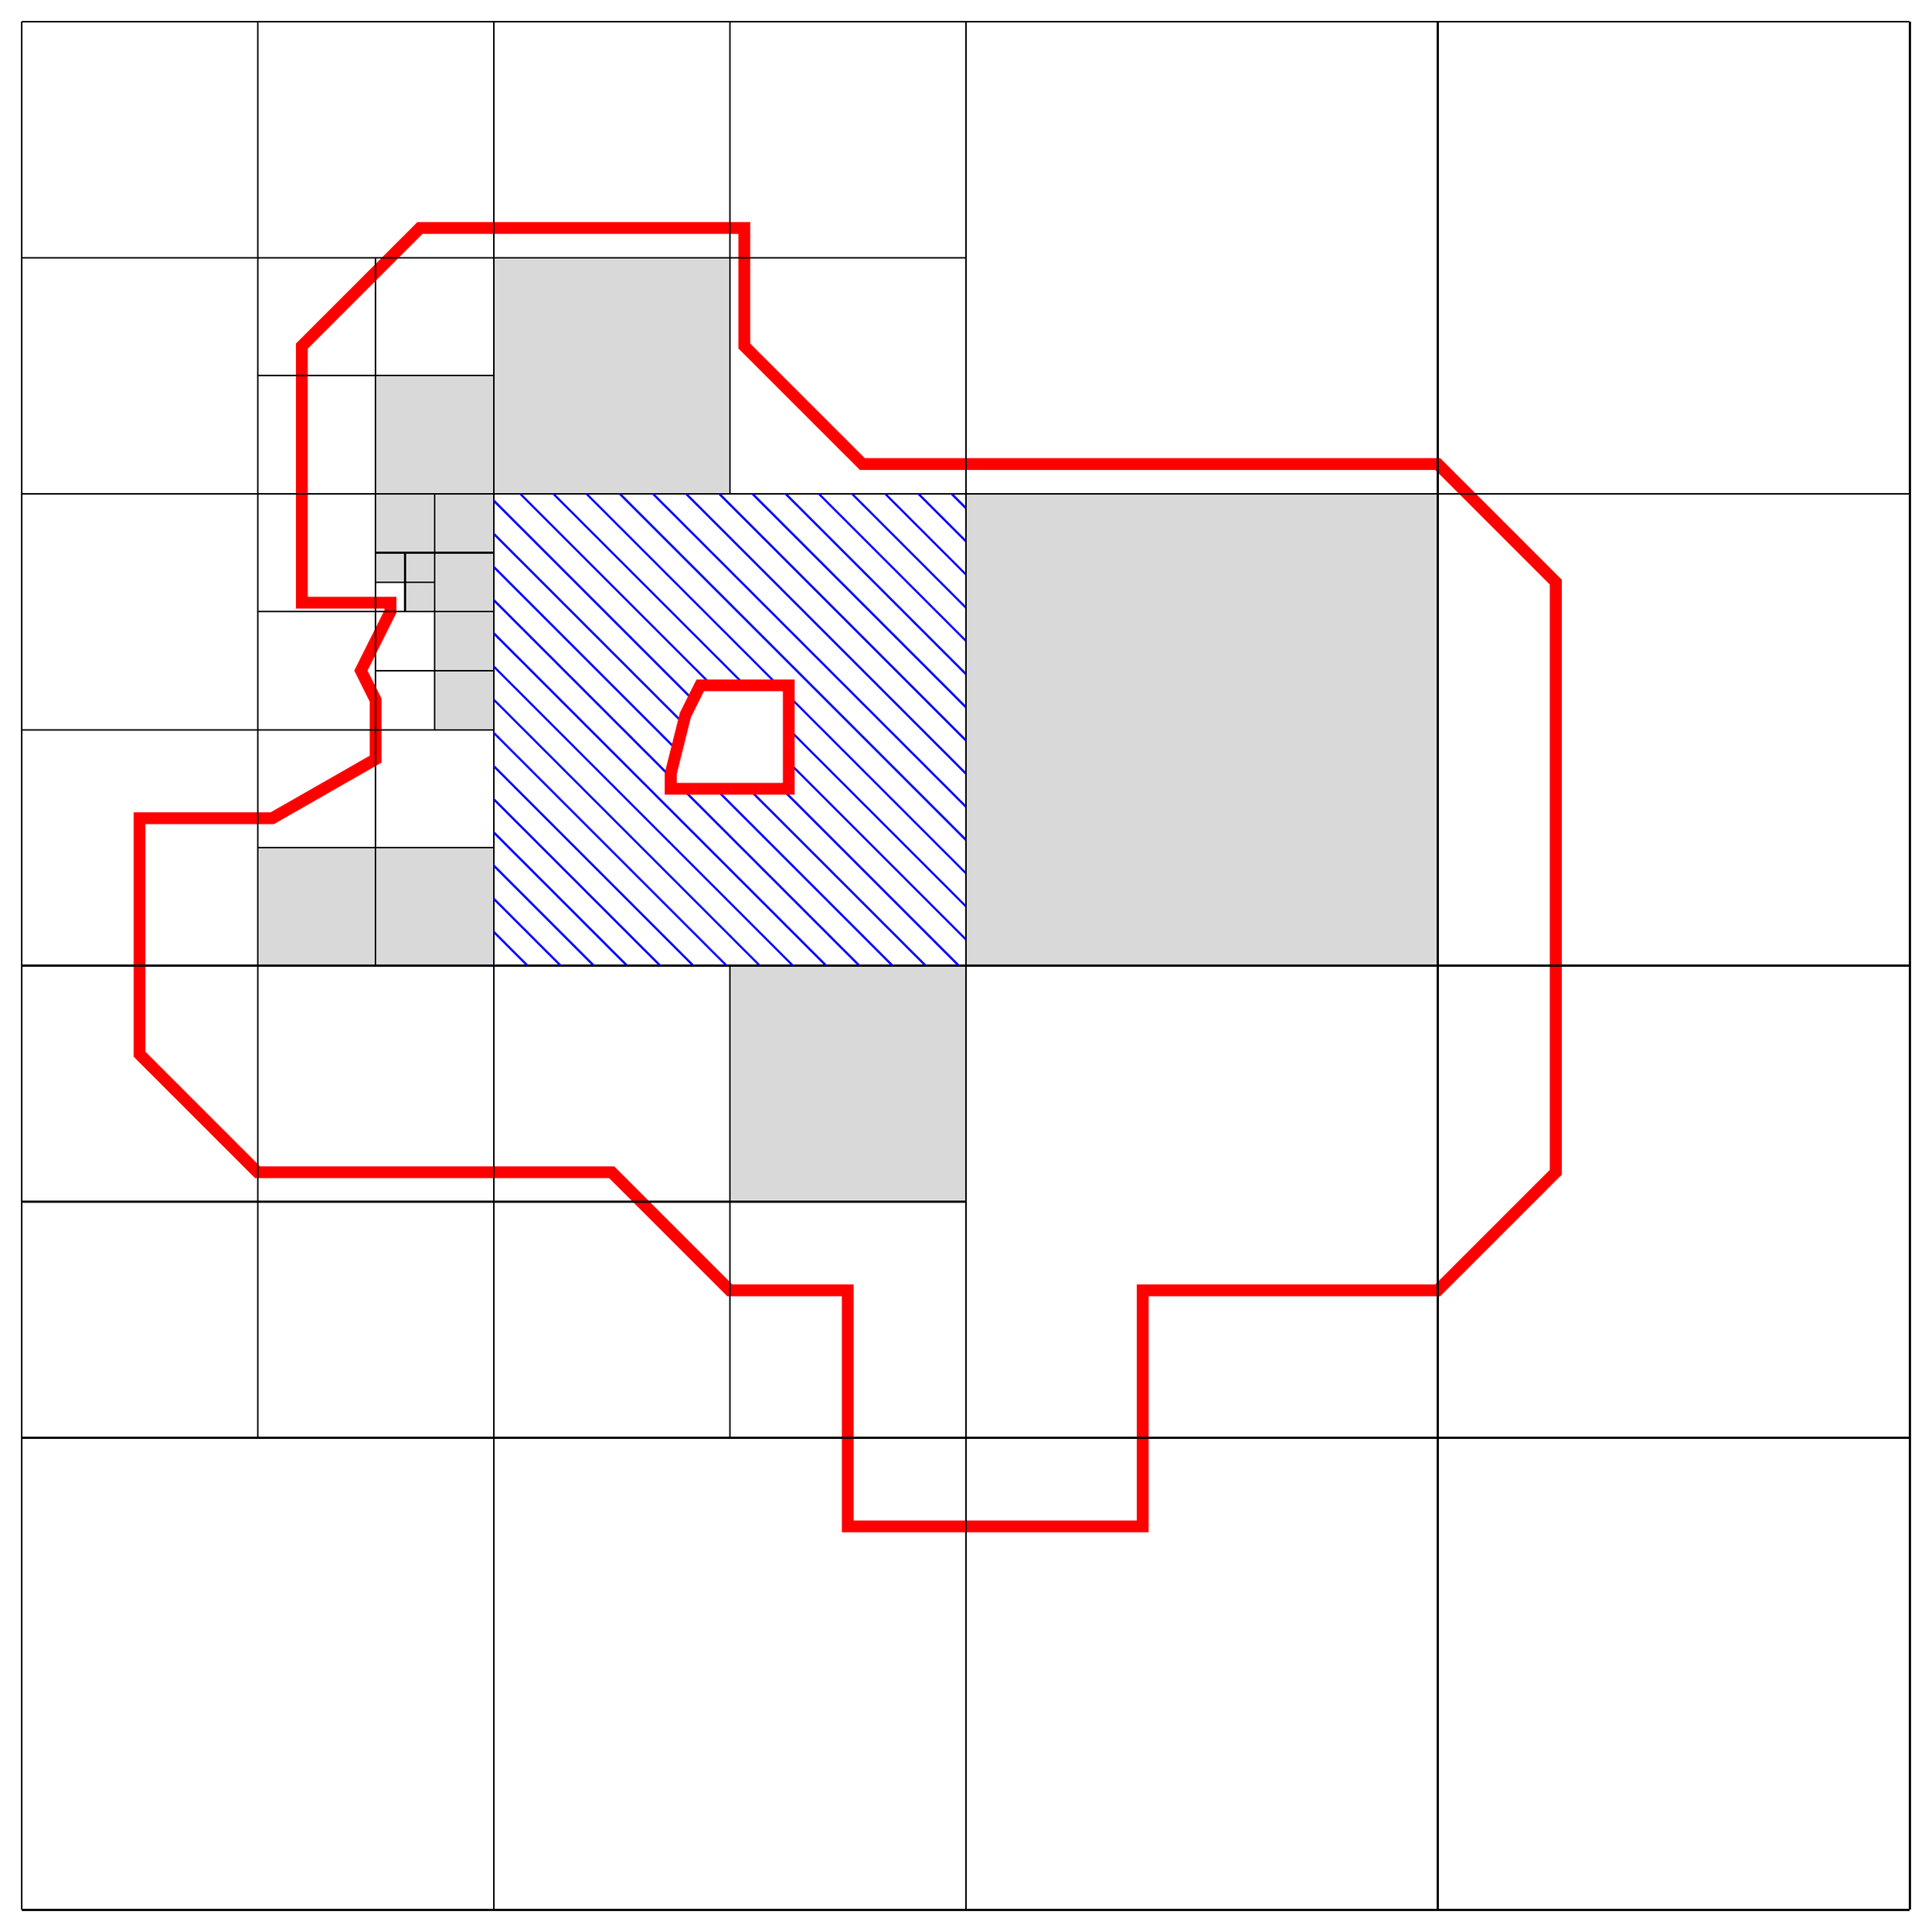
\begin{tikzpicture}
        %\draw[step=1, very thin, light-gray, dashed] (0,0) grid (32,32);
        
        \node (start) at (6.25,22.25) {};
        \draw[poly] (start) -- ++(0,-0.25) -- ++(-0.25,-0.5) -- ++(-0.25,-0.5)  -- ++(0.25,-0.5)
            -- ++(0,-1) -- ++(-1.75,-1) -- ++(-2.25,0) -- ++(0,-4) -- ++(2,-2)
            -- ++(6,0) -- ++(2,-2) -- ++(2,0) -- ++(0,-4) -- ++(5,0) -- ++(0,4) -- ++(5,0) 
            -- ++(2,2) -- ++(0,10) -- ++(-2,2) -- ++(-9.75,0) -- ++(-2,2) 
            -- ++(0,2) -- ++(-5.5,0) -- ++(-2,-2) -- ++(0,-4.35) -- ++(1.6,0);
        \draw[step=8,  thick, black] (0,0)  grid (32,32);
        \draw[step=4,  thick, black] (0,24) grid (8,32);
        \draw[step=4,  thick, black] (0,16) grid (8,24);
        \draw[step=4,  thick, black] (0,8)  grid (8,16);
        \draw[step=4,  thick, black] (8,8)  grid (16,16);
        \draw[step=4,  thick, black] (8,24) grid (16,32);
        \draw[step=2,  thick, black] (4,16) grid (8,20);
        \draw[step=2,  thick, black] (4,20) grid (8,24);
        \draw[step=2,  thick, black] (4,24) grid (8,28);
        \draw[step=1,  thick, black] (6,20) grid (8,24);
        \draw[step=0.5,thick, black] (6,22) grid (7,23);

        \draw[pattern=custom north west lines,hatchspread=16pt,hatchthickness=1pt,hatchcolor=blue] (8,16) rectangle (16,24);

        \draw[shadow1] (16,16) rectangle (24,24);
        \draw[shadow1] (6,16) rectangle (8,18);
        \draw[shadow1] (4,16) rectangle (6,18);
        \draw[shadow1] (12,12) rectangle (16,16);
        \draw[shadow1] (8,24) rectangle (12,28);
        \draw[shadow1] (6,24) rectangle (8,26);        
        \draw[shadow1] (6,23) rectangle (7,24);
        \draw[shadow1] (7,23) rectangle (8,24);
        \draw[shadow1] (7,22) rectangle (8,23);
        \draw[shadow1] (7,21) rectangle (8,22);
        \draw[shadow1] (7,20) rectangle (8,21);
        \draw[shadow1] (6,22.5) rectangle (6.5,23);
        \draw[shadow1] (6.5,22.5) rectangle (7,23);
        \draw[shadow1] (6.5,22) rectangle (7,22.5);
        
        \draw[white, fill] (11,19) -- ++(0,0.25) -- ++(0.25,1) -- ++(0.25,0.5)
            --++(1.5,0) --++(0,-1.75) --++(-2.1,0);
        \draw[poly] (11,19) -- ++(0,0.25) -- ++(0.25,1) -- ++(0.25,0.5)
            --++(1.5,0) --++(0,-1.75) --++(-2.1,0);
        
    \end{tikzpicture}
\end{page}
\end{document} 
